%% LyX 2.4.4 created this file.  For more info, see https://www.lyx.org/.
%% Do not edit unless you really know what you are doing.
\documentclass[english,american]{article}
\usepackage[T1]{fontenc}
\usepackage[utf8]{inputenc}
\usepackage{babel}
\usepackage{varwidth}
\usepackage{amssymb}
\usepackage{graphicx}
\usepackage[]
 {hyperref}

\makeatletter

%%%%%%%%%%%%%%%%%%%%%%%%%%%%%% LyX specific LaTeX commands.
%% Because html converters don't know tabularnewline
\providecommand{\tabularnewline}{\\}
%% Variable width box for table cells
\newenvironment{cellvarwidth}[1][t]
    {\begin{varwidth}[#1]{\linewidth}}
    {\@finalstrut\@arstrutbox\end{varwidth}}

\makeatother

\usepackage{listings}
\usepackage[bibstyle=trad-unsrt,citestyle=numeric]{biblatex}
\addto\captionsamerican{\renewcommand{\lstlistingname}{\protect\inputencoding{latin9}Listing}}
\addto\captionsenglish{\renewcommand{\lstlistingname}{\protect\inputencoding{latin9}Listing}}
\renewcommand{\lstlistingname}{\protect\inputencoding{latin9}Listing}

\addbibresource{biocpy_references.bib}
\begin{document}
\title{BiocPy: A Comprehensive Framework for Cross-Platform Genomic Interoperability
and Polyglot Workflows}
\author{Jayaram Kancherla\textsuperscript{\selectlanguage{english}%
1}, Aaron T.L. Lun\textsuperscript{2}\\
\textsuperscript{\selectlanguage{english}%
1}Genentech Inc., South San Francisco, CA, USA\\
\textsuperscript{2}Aarun Lun Inc, Sydney, Australia}

\maketitle
The modern landscape of computational biology is characterized by
two main ecosystems: the statistical methods available through Bioconductor,
rooted in the R programming language, and the rapid growth of machine
learning frameworks within the Python ecosystem. Bioconductor has
served as the gold standard for high-throughput genomic analysis by
providing standardized data structures and reproducible statistical
methods, where as Python has quickly become the primary environment
for deep learning, image analysis, and general-purpose data science.
This presents a challenge to the scientific community, navigating
complex, fragile, and often inefficient interoperability solutions
to leverage the strengths of both worlds.

We present BiocPy, a software framework and ecosystem designed to
bridge this gap. BiocPy is not a wrapper for R functions rather, it
re-engineers the foundational data structures of Bioconductor, specifically
GenomicRanges, SummarizedExperiment, SingleCellExperiment etc. as
native Python data representations. Furthermore, BiocPy provides the
rds2py package facilitating the direct ingestion of serialized R data
objects (RDS files) into Python environments. Using BiocPy's data
structures enables seamless, polyglot analysis workflows for e.g.
the scran/singleR collection of tools for single-cell RNA-seq analysis.
All packages in the BiocPy ecosystem are published to Python's Package
Index (PyPI) \href{http://github.com/BiocPy}{http://github.com/BiocPy}.

\section{Introduction}

Bioinformatics is an interdisciplinary field at the intersection of
molecular biology, statistics, and computer science. Historically,
these disciplines have favored different computational tools, leading
to a diverse software landscape to perform genomic analyses. Bioconductor\cite{gentleman_bioconductor_2004}
built upon the R programming language, it was designed with a primary
focus on statistical analysis and visualization of genomic data. Over
the last two decades, it has grown into a repository of over 2,000
packages, conforming to a strict set of shared data structures and
design principles. The strength of Bioconductor lies in its community-driven
standardization and peer-review process, objects such as GenomicRanges\cite{lawrence_software_2013}
and SummarizedExperiment\cite{noauthor_summarizedexperiment_nodate}
provide a common currency for data exchange, allowing developers to
quickly build and iterate methods without reinventing new data structures.
For researchers focused on rigorous statistical testing methods and
established genomic workflows, Bioconductor remains the standard environment
to perform these analyses. 

Python has emerged over the last decade as the dominant language of
data science and machine learning (ML). Powered by libraries such
as NumPy\cite{harris_array_2020}, PyTorch\cite{paszke_pytorch_2019},
and TensorFlow\cite{abadi_tensorflow_2016}, it provides flexibility,
and integration with modern computing paradigms (distributed computing,
ease of GPU access etc). In the context of genomics, Python has seen
a surge in popularity driven by the rise of single-cell analysis through
the scverse efforts\cite{virshup_scverse_2023}, where large-scale
analyses benefit significantly from ML libraries (e.g. rapids-singlecell\cite{dicks_scverserapids_singlecell_2024}).

The coexistence of these two powerful computational ecosystems creates
a fragmentation problem. A typical modern genomic workflow might require
the robust methods available in Bioconductor (R), followed by the
application of a deep learning models or inference methods available
in Python. Traditionally, researchers navigated this by:
\begin{itemize}
\item \textbf{File-based exchange: }Saving intermediate results in CSV or
text files. This is error-prone, loses metadata, and is computationally
expensive due to repeated serialization and deserialization when dealing
with a large cohort of samples.
\item \textbf{Interface libraries: }Using tools like rpy2\cite{noauthor_rpy2rpy2_2025}
to run R code within Python. While functional, rpy2 requires the user
to maintain two complex runtime environments (R and Python) simultaneously,
leading to dependency hell, installation fragility, and significant
overhead in context switching.
\item \textbf{Reimplementation: }Rewriting statistical methods in Python.
This often leads to subtle differences in results, lacks the peer-reviewed
rigor of the original Bioconductor implementation, and contributes
to incompatibility in standard data models (e.g., the divergence between
Bioconductor's SingleCellExperiment\cite{amezquita_orchestrating_2020}
and scverse's AnnData\cite{virshup_anndata_2024}).
\end{itemize}
BiocPy addresses this gap, rather than forcing R to run inside Python
(vice-versa), or creating an entirely new, incompatible Python-native
standard, BiocPy ports Bioconductor’s core class definitions into
Python. A SummarizedExperiment in BiocPy is designed to have the same
slots, and the same behavioral guarantees as its R counterpart. This
ensures that the conceptual data model remains consistent, reducing
the cognitive burden for researchers transitioning between languages.
By adhering to Bioconductor’s design principles, such as the separation
of assay data from row/column metadata and the use of functional programming
patterns, BiocPy enables a workflow where data can round-trip between
R and Python. Furthermore, By providing Python bindings to these same
C++ libraries (e.g., libscran\cite{noauthor_libscran_nodate}), BiocPy
allows Python users to access the exact same methods in R, ensuring
consistent interpretation and reliability in results. These efforts
create a bridge between computational platforms and enables researches
to focus their time on biological questions rather than technical
challenges.

BiocPy is not the only attempt to solve the R/Python divide, but its
approach is unique. Unlike rpy2, which is powerful but heavy due to
embedding an R instance, it's often difficult to configure in containerized
environments (Docker/Singularity). BiocPy is lightweight and native.
AnnData is excellent for single-cell matrices but lacks the generality
of SummarizedExperiment (which handles any matrix data) and does not
support GenomicRanges (or range based operations). BiocPy supports
a broader spectrum of genomic data types. Finally, while writing genomic
tools in pure Python is possible, it often leads to poor performance
or lack of standardization; BiocPy provides the necessary structure
for stable and sustainable software development.
\begin{center}
\begin{figure}[h]
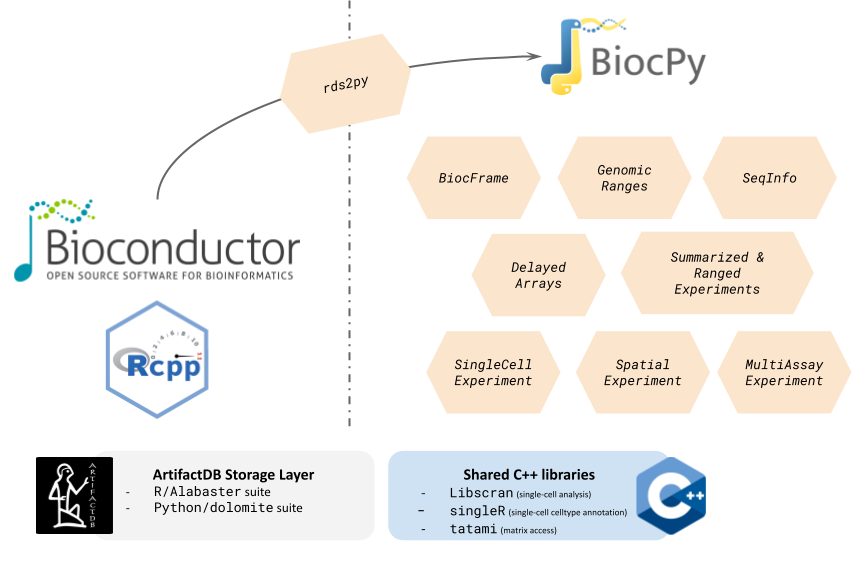
\includegraphics[scale=0.4]{main_figure}

\caption{Overview of the BiocPy framework. BiocPy provides native Python implementations
of core Bioconductor classes, enabling shared memory representations
and direct interoperability with R data artifacts. This figure illustrates
the parallel class structures between Bioconductor and BiocPy along
with shared C++ backends (e.g., libscran) and interoperability storage
layers (rds2py, ArtifactDB).}
\end{figure}
\par\end{center}

\section{Core Data Structures}

The development of BiocPy is not just a translation of R code into
Python, it is adoption of Bioconductor’s design philosophy into a
Pythonic context. The development of the ecosystem is guided by adherence
to specific design principles that prioritize reliability, interoperability
and usability.
\begin{itemize}
\item \textbf{Functional Programming and Immutability: }An important feature
of the BiocPy ecosystem is its reliance on functional programming
paradigms. In the broader Python data science world, libraries like
pandas\cite{mckinney_pandas_nodate} often encourage in-place modification
of objects (e.g., df.drop(..., inplace=True)). While convenient for
simple scripts, in-place mutation can be dangerous in complex genomic
pipelines where multiple analysis steps reference the same underlying
data object. Side effects from one function can inadvertently corrupt
the state of the data for downstream processes. BiocPy mitigates this
by adopting a functional approach similar to R. Operations that modify
an object typically return a new instance rather than altering the
original. This approach enhances the safety of modular workflows,
ensuring that the input data remains invariant unless explicitly overwritten.
\item \textbf{Python-Native Implementation with Minimal Dependencies: }While
the conceptual architecture borrows from R, the implementation is
strictly Python-native. BiocPy leverages the well established scientific
Python stack, NumPy for numerical arrays, SciPy\cite{virtanen_scipy_2020}
for sparse matrices, to ensure high performance and compatibility.
The ecosystem maintains a lean dependency footprint. By avoiding unnecessary
heavy libraries, BiocPy ensures that its core packages (BiocFrame,
GenomicRanges, SummarizedExperiment) can be installed easily in diverse
environments. This lightweight design facilitates the creation of
clean environments using Conda or pip, minimizing the dependency conflicts
that plague complex bioinformatics software stacks.
\end{itemize}

\subsection{BiocFrame: A Flexible DataFrame}

The pandas DataFrame is ubiquitous in most analysis workflows. However,
for genomic data, pandas presents several limitations that BiocFrame
addresses.
\begin{itemize}
\item \textbf{Type Preservation: }One of the most persistent issues with
pandas in a bioinformatics context is its aggressive type inference
and coercion. For example, introducing a missing value (NaN) into
an integer column in pandas typically forces the entire column to
be cast to floating-point, as integer type does not support NaN. In
genomics, the distinction between an integer count of 0, a count of
1, and a missing value is critical. BiocFrame follows the Bioconductor
principle of \textquotedbl what you put is what you get\textquotedbl .
It preserves the original data types of columns, ensuring that integer
counts remain integers and that complex objects are stored as intended.
This type stability is crucial when the data represents biological
measurements.
\item \textbf{Nested and Complex Data: }Genomic data is rarely flat. A single
row representing a gene might have multiple associated pieces of metadata
that are themselves lists or complex objects (e.g., a list of exons,
a set of protein domains, or a GenomicRanges object representing its
locus). pandas generally struggles with columns containing complex
objects, often relegating them to a slow, generic object dtype. BiocFrame
is designed to support nested data structures natively. It can hold
columns that are themselves BiocFrame objects or lists of varying
lengths. This allows for the construction of recursive, hierarchical
models that accurately reflect the biological data, rather than flattening
everything into a 2D table.
\item \textbf{Functional Programming Paradigm: }As mentioned in the design
philosophy, BiocPy, mirroring Bioconductor, adopts a functional programming
paradigm. BiocFrame operations typically return new objects. This
immutability-by-default approach, while different from standard Pythonic
patterns, is safer for complex scientific pipelines where tracking
the state of data is important. This applies not only to BiocFrame
but all packages within BiocPy.
\end{itemize}
\bgroup\inputencoding{latin9}
\begin{lstlisting}[language=Python,numbers=left,showstringspaces=false]
from biocframe import BiocFrame

# A BiocFrame can hold complex, nested lists natively
bframe = BiocFrame ({
	"gene_id": ["G1", "G2", "G3"],
	"counts": [10, 20, None],
	"isoforms": [["iso1", "iso2"], ["iso3"], 
		["iso4", "iso5", "iso6"]],
	"location": BiocFrame({
        "chromosome": ["chr17", "chr17", "chr7"],
        "start": [43044295, 7668422, 55019017],
        "end": [43125483, 7687550, 55211628],
        "strand": ["-", "-", "+"],
    }),
})

print(bframe)

# Chain operations without side effects
# All operations return new objects
modified = (bframe
    .set_column_names(["gene_id", "expression_counts", 
		"isoforms", "locations"])
    .set_row_names(["row1", "row2", "row3"])
    .set_metadata({"source": "example"})
)

# Original is unchanged
print("Original column names:", bframe.column_names)
print("Modified column names:", modified.column_names)
\end{lstlisting}
\leavevmode\egroup

\bgroup\inputencoding{latin9}
\begin{lstlisting}[showstringspaces=false]
## OUTPUT
# ... nested structures are preserved without object -dtype coercion
BiocFrame with 3 rows and 4 columns
    gene_id  counts                 isoforms                   location
      <list>  <list>                   <list>               <BiocFrame>
[0]       G1      10         ['iso1', 'iso2'] chr17:43044295:43125483:-
[1]       G2      20                 ['iso3']   chr17:7668422:7687550:-
[2]       G3    None ['iso4', 'iso5', 'iso6']  chr7:55019017:55211628:+


Original column names: ['gene_id', 'counts', 'isoforms', 'location']
Modified column names: ['gene_id', 'expression_counts', 'isoforms', 'locations']
\end{lstlisting}
\leavevmode\egroup

Additionally, BiocFrame includes robust utilities for conversion to
and from pandas or polar objects, because researchers often need to
leverage these for general data cleaning or visualization tasks before
moving into Bioconductor-specific workflows.

\subsection{GenomicRanges}

The most crucial feature of Bioconductor is its handling of genomic
intervals via the GenomicRanges package. In Python, interval arithmetic
has historically been handled by wrapping command-line tools (like
bedtools\cite{quinlan_bedtools_2010}) or using standalone libraries
like pyranges. BiocPy brings a native, in-memory implementation of
GenomicRanges to Python. The BiocPy implementation decomposes genomic
information into three interacting classes:
\begin{itemize}
\item \textbf{Sequence Information: }Stores the \textquotedbl universe\textquotedbl{}
of the experiment, the chromosome names and their lengths. This prevents
invalid operations, such as defining a range that extends beyond the
end of a chromosome.
\item \textbf{Ranges:} Implements generic integer interval arithmetic. This
calculates overlaps, gaps, and shifts, independent of biological context.
\item \textbf{Genomic metadata: }Adds the biological layer, chromosome names
(sequence names) and strand information (+, -, or {*}) to the IRanges.
\end{itemize}
BiocPy’s GenomicRanges abstracts the coordinate system, providing
methods to import from commonly used annotation file formats or R
objects while maintaining internal consistency. The availability of
methods like findOverlaps, nearest, and resize in native Python allows
for complex analyses. For example, one can load a set of ChIP-seq
peaks and a set of gene annotations, and in a few lines of Python,
determine which genes have peaks in their promoter regions, handling
strand-specificity automatically.

\subsection{Containers for Experimental Data}

To encapsulate the complexity of high-throughput experiments, BiocPy
provides container classes that bind assay data to metadata.
\begin{itemize}
\item \textbf{SummarizedExperiment: }The SummarizedExperiment (SE) class
is the fundamental container for matrix-like data. It enforces a strict
geometry:
\begin{itemize}
\item \textbf{Assays: }A list of matrices (e.g., counts, log-counts) where
rows are features and columns are samples.
\item \textbf{RowData: }A BiocFrame (or GenomicRanges in the case of RangedSummarizedExperiment
{[}rowRanges{]}) describing the rows. Must match the number of rows
in assays.
\item \textbf{ColData: }A BiocFrame describing the columns (samples). Must
match the number of columns in assays.
\end{itemize}
\item \textbf{SingleCellExperiment: }Extending SE, the SingleCellExperiment
(SCE) is tailored for scRNA-seq. It adds slots for:
\begin{itemize}
\item \textbf{ReducedDims: }Storing embeddings like PCA, t-SNE, and UMAP
coordinates directly within the object.
\item \textbf{AltExps: }Storing \textquotedbl Alternative Experiments.\textquotedbl{}
In modern single-cell workflows, a cell might have RNA data, but also
Spike-in controls, or Antibody Derived Tags (CITE-seq). AltExps allows
these auxiliary matrices to be stored within the main object, linked
to the same cells but with different feature sets.
\end{itemize}
This design contrasts with the AnnData object used in scverse (scanpy)
ecosystem. While AnnData is powerful, SingleCellExperiment offers
a stricter adherence to the Bioconductor S4 model, support genomic
range operations and facilitating interoperability with R tools.
\item \textbf{MultiAssayExperiment: }For complex study designs involving
multiple assays performed on the same subjects (e.g., a cohort with
RNA-seq, mutation calls, and copy number variants), BiocPy implements
MultiAssayExperiment\cite{noauthor_software_nodate}. This container
manages a collection of experiments (which can be SummarizedExperiment
objects or its derivatives) and a sample map that links biological
specimens to the specific assays performed on them. This structure
is vital for multi-omics integration, allowing for coordinated subsetting
across diverse data modalities.
\end{itemize}
And many more packages for efficiently handling and lazily operating
on data on-disk (delayed arrays), and extending summarized experiment
representations to support spatial modalities as shown in Table 1. 
\begin{center}
\begin{table}[h]
\centering
\begin{tabular}{|c|c|c|}
\hline 
 & \textbf{Bioconductor} & \textbf{BiocPy}\tabularnewline
\hline 
\multicolumn{1}{c}{\textbf{Base Data Structures}} & \multicolumn{1}{c}{} & \multicolumn{1}{c}{}\tabularnewline
\hline 
Data Frame & \begin{cellvarwidth}[t]
\centering
Supported by DataFrame 

\& DFrame classes
\end{cellvarwidth} & BiocFrame\tabularnewline
\hline 
IRanges & $\checkmark$ & $\checkmark$\tabularnewline
\hline 
GenomicRanges & $\checkmark$ & $\checkmark$\tabularnewline
\hline 
\multicolumn{1}{c}{\textbf{Experiment Containers}} & \multicolumn{1}{c}{} & \multicolumn{1}{c}{}\tabularnewline
\hline 
SummarizedExperiment & $\checkmark$ & $\checkmark$\tabularnewline
\hline 
SingleCellExperiment & $\checkmark$ & $\checkmark$\tabularnewline
\hline 
MultiAssayExperiment & $\checkmark$ & $\checkmark$\tabularnewline
\hline 
SpatialFeatureExperiment & $\checkmark$ & $\checkmark$\tabularnewline
\hline 
SpatialExperiment & $\checkmark$ & $\checkmark$\tabularnewline
\hline 
\multicolumn{1}{c}{\textbf{Utilities \& R Interoperability}} & \multicolumn{1}{c}{} & \multicolumn{1}{c}{}\tabularnewline
\hline 
rds2py & -- & $\checkmark$\tabularnewline
\hline 
ArtifactDB representations & $\checkmark$ (package: alabaster) & $\checkmark$ (package: dolomite)\tabularnewline
\hline 
BiocUtils & \begin{cellvarwidth}[t]
\centering
Common utilities mirroring 

R's base functionality
\end{cellvarwidth} & $\checkmark$\tabularnewline
\hline 
mopsy & \begin{cellvarwidth}[t]
\centering
Matrix operations with 

R-like syntax
\end{cellvarwidth} & $\checkmark$\tabularnewline
\hline 
BiocFileCache & $\checkmark$ & $\checkmark$\tabularnewline
\hline 
\multicolumn{1}{c}{\textbf{Delayed Operations}} & \multicolumn{1}{c}{} & \multicolumn{1}{c}{}\tabularnewline
\hline 
DelayedArray & $\checkmark$ & $\checkmark$\tabularnewline
\hline 
HDF5Array & $\checkmark$ & $\checkmark$\tabularnewline
\hline 
TileDBArray & $\checkmark$ & $\checkmark$\tabularnewline
\hline 
\multicolumn{1}{c}{\textbf{Analysis methods}} & \multicolumn{1}{c}{} & \multicolumn{1}{c}{}\tabularnewline
\hline 
\begin{cellvarwidth}[t]
\centering
scran - Multi-model 

single-cell analysis
\end{cellvarwidth} & $\checkmark$ (package: scrapper) & $\checkmark$ (package: scranpy)\tabularnewline
\hline 
\begin{cellvarwidth}[t]
\centering
SingleR: Cell type 

annotation
\end{cellvarwidth} & $\checkmark$ (package: singleR) & $\checkmark$ (package: singler)\tabularnewline
\hline 
\end{tabular}

\caption{List of Bioconductor equivalent BiocPy packages. }

\end{table}
\par\end{center}

\section{Interoperability}

A major barrier in cross-language workflows is the incompatibility
of data serialization formats (R’s RDS vs. Python’s Pickle). BiocPy
addresses this challenge through two primary approaches: direct binary
ingestion via rds2py and language-agnostic interchange via ArtifactDB.

\subsection{Direct Ingestion with rds2py}

BiocPy provides rds2py, a package that can read R’s binary serialization
format (RDS). This allows Python environments to ingest complex S4
objects directly from disk without requiring an installed R runtime.
rds2py implements memory-efficient loading strategies rather than
performing deep copies where ever possible. This is essential when
loading large Bioconductor objects for downstream analyses in Python.

\bgroup\inputencoding{latin9}
\begin{lstlisting}[language=Python,numbers=left,showstringspaces=false]
from rds2py import read_rds

# Load a pre - processed R object (e.g., from a colleague )
r_obj = read_rds("processed_data.rds")

# uses BiocPy's SingleCellExperiment representation
print(sce)
\end{lstlisting}
\leavevmode\egroup

\bgroup\inputencoding{latin9}
\begin{lstlisting}
## OUTPUT
class: SingleCellExperiment
dimensions: (20006, 2874)
assays(2): ['counts', 'logcounts']
row_data columns(0): []
row_names(0):  
column_data columns(15): ['tissue', 'group #', 
'total mRNA mol', ..., 'subsets.Mito', 'sizeFactor', 'label']
column_names(2874): ['1772071015_C02', '1772071017_G12', 
'1772071017_A05', ..., '1772066097_D04', '1772063068_D01', 
'1772066098_A12']
main_experiment_name:  
reduced_dims(0): []
alternative_experiments(2): ['ERCC', 'repeat']
row_pairs(0): []
column_pairs(0): []
metadata(0): 
\end{lstlisting}
\leavevmode\egroup


\subsection{Language-Agnostic Formats with ArtifactDB}

For sustainable collaborative workflows across computational environments,
BiocPy integrates with language agnostic schemas and specifications
defined in ArtifactDB\cite{noauthor_artifactdb_nodate}. ArtifactDB
is a system for managing genomic datasets on-disk where data is stored
in language-neutral formats (HDF5 for matrices, JSON for metadata
etc) but is wrapped in rich semantic metadata. ArtifactDB validates
these objects to ensure cross language accessibility of the data.

This layer acts as an intermediate exchange format. An R user can
serialize a SingleCellExperiment to disk using ArtifactDB, and a Python
user can fetch that same artifact from disk. The ArtifactDB python
clients automatically reconstructs the native Python object from the
remote components using an appropriate BiocPy class. This ensures
that datasets remain consistent across the research community, regardless
of the programming language used for analysis.

\bgroup\inputencoding{latin9}
\begin{lstlisting}[language=R,numbers=left,showstringspaces=false]
# R code
library(SingleCellExperiment)
example(SingleCellExperiment, echo=FALSE)

library(alabaster.sce)
path <- "/my/data/path"
saveObject(sce, path)
\end{lstlisting}
\leavevmode\egroup

\bgroup\inputencoding{latin9}
\begin{lstlisting}[language=Python,numbers=left,showstringspaces=false]
# Python code
import dolomite_base

path = "/my/data/path"
out = dolomite_base.read_object(path)
print(out)
\end{lstlisting}
\leavevmode\egroup
\bgroup\inputencoding{latin9}
\begin{lstlisting}
##OUTPUT
class: SingleCellExperiment
dimensions: (200 100)
assays(2): ['counts', 'logcounts']
row_data columns(0): []
row_names(0):  
column_data columns(0): []
column_names(0): []
main_experiment_name:  
reduced_dims(0): []
alternative_experiments(0): []
row_pairs(0): []
column_pairs(0): []
metadata(0): 
\end{lstlisting}
\leavevmode\egroup

\begin{quote}
Note: The library names ``alabaster'' and ``dolomite'' are the
manifestations of the ArtifactDB schemas and specifications in R and
Python respectively.
\end{quote}
The scrnaseq\cite{noauthor_singler-inccelldex-py_2025,noauthor_singler-inccelldex_2025}
(collection of single-cell RNA-seq datasets) and celldex\cite{noauthor_singler-inccelldex-py_2025,noauthor_singler-inccelldex_2025}
(collection of reference single-cell datasets for cell type annotation)
repositories store their data in ArtifactDB format, providing access
to these resources in both R and Python. 

\subsection{Integration with Broader Python Ecosystem}

BiocPy acts as a central hub, not just connecting to R but also to
the broader Python ecosystem. We take advantage of existing efforts
in Python whenever possible
\begin{itemize}
\item \textbf{scverse: }The AnnData format is the standard for the scverse
ecosystem (scanpy). BiocPy provides utilities to convert SingleCellExperiment
objects to AnnData objects. This allows users to mix and match tools:
utilizing Bioconductor’s statistical methods for normalization and
feature selection, then converting to AnnData to use Scanpy’s visualization
tools or scvi-tools for probabilistic modeling.
\item \textbf{Pandas or Polars: }As noted in the BiocFrame section, the
integration with pandas ensures that BiocPy objects can easily interface
with general-purpose data cleaning and visualization libraries.
\end{itemize}

\section{Enabling Methods Development and Polyglot Workflows}

The true value of BiocPy lies not just in data representations and
storage, but in enabling robust methods development and flexible,
iterative analysis pipelines. By providing standard data structures
and shared C++ backends, BiocPy allows developers to build tools that
are reproducible across languages and allows analysts to leverage
the best of both worlds.

\subsection{Shared C++ libraries}

\subsubsection{Multi-modal Single-Cell Analysis using scranpy}

Reproducibility is often compromised when methods are re-implemented
in different languages due to subtle differences in algorithms. BiocPy
addresses this by binding to the same standalone C++ libraries used
by R packages. For example, the scran\cite{lun_step-by-step_2016}/scrapper\cite{noauthor_scrapper_nodate,lun_powering_2023}
package is a staple of scRNA-seq analysis in R\cite{amezquita_orchestrating_2020}.
Its core logic resides in libscran, a C++ library. BiocPy’s scranpy
links to this same library. When a user performs log-normalization
or feature selection in Python using scranpy, they are executing the
exact same compiled code as an R user. This guarantees that the statistical
transformations applied to the data are identical, preserving the
validity of downstream comparisons.

\bgroup\inputencoding{latin9}
\begin{lstlisting}[language=Python,numbers=left,showstringspaces=false]
import scranpy
from singlecellexperiment import SingleCellExperiment
from scipy import sparse
import numpy as np
from rds2py import read_rds

# Download the test dataset from 
# [here](https://github.com/kanaverse/random-test-files/releases) 
# or pick your own dataset
# We choose the ziesel brain dataset
sce = read_rds("csc.rds") 
print(sce)

# Run full scran analysis with defaults
results = scranpy.analyze(sce)

# Access the normalized counts
print(results.rna_normalized)

# Convert analysis results to a SingleCellExperiment
print(results.to_singlecellexperiment())
\end{lstlisting}
\leavevmode\egroup

\bgroup\inputencoding{latin9}
\begin{lstlisting}[showstringspaces=false]
## OUTPUT
class: SingleCellExperiment
dimensions: (20006, 3005)
assays(1): ['counts']
row_data columns(0): []
row_names(0):  
column_data columns(10): ['tissue', 'group #', 
'total mRNA mol', 'well', 'sex', 'age', 'diameter', 
'cell_id', 'level1class', 'level2class']
column_names(3005): ['1772071015_C02', '1772071017_G12', 
'1772071017_A05', ..., '1772063068_D01', '1772066098_A12',
'1772058148_F03']
main_experiment_name:  
reduced_dims(0): []
alternative_experiments(2): ['ERCC', 'repeat']
row_pairs(0): []
column_pairs(0): []
metadata(0): 

# normalized counts
<20006 x 3002> DelayedArray object of type 'float64'
[[0.        , 0.        , 0.        , ..., 0.        , 0.        ,
  1.71829137],
 [1.58903752, 0.72632423, 0.        , ..., 0.        , 0.        ,
  1.71829137],
 [1.58903752, 0.72632423, 1.90880006, ..., 0.        , 0.        ,
  0.        ],
 ...,
 [6.73850101, 7.74376021, 6.59938726, ..., 9.17864868, 7.45000363,
  9.68523385],
 [4.44323218, 5.87255369, 5.50901887, ..., 7.23715052, 5.88144921,
  6.9081424 ],
 [3.27849603, 3.34509245, 2.35964763, ..., 5.78012009, 3.95306026,
  4.94373579]]

# with results
class: SingleCellExperiment
dimensions: (20006, 3002)
assays(2): ['filtered', 'normalized']
row_data columns(5): ['mean', 'variance', 'fitted', 
'residual', 'is_highly_variable']
row_names(0):  
column_data columns(4): ['sum', 'detected', 'size_factors', 
'clusters']
column_names(3002): ['1772071015_C02', '1772071017_G12', 
'1772071017_A05', ..., '1772063068_D01', '1772066098_A12', 
'1772058148_F03']
main_experiment_name:  
reduced_dims(3): ['pca', 'tsne', 'umap']
alternative_experiments(0): []
row_pairs(0): []
column_pairs(0): []
metadata(0): 
\end{lstlisting}
\leavevmode\egroup


\subsubsection{SingleR: Reference-Based Annotation}

Cell type annotation is a critical step in single-cell analysis. We
demonstrate how BiocPy enables the use of Bioconductor’s reference-based
annotation tools directly within a Python environment, using the singler\cite{aran_reference-based_2019,noauthor_singler-inc_nodate}
package. This workflow highlights the ecosystem’s ability to fetch
remote references and apply rigorous statistical methods, using the
exact same algorithms available in R.

\bgroup\inputencoding{latin9}
\begin{lstlisting}[language=Python,showstringspaces=false]
import celldex
import singler
from rds2py import read_rds
from singlecellexperiment import SingleCellExperiment
import scrnaseq

# Load Query Data (e.g., processed in R or Python)
# Ingest a standard anndata object containing log-counts
sce = SingleCellExperiment.from_anndata("pbmc_10k.h5ad")

# Fetch Reference Data
# Seamlessly download versioned Bioconductor references
# This returns a SummarizedExperiment object
ref = celldex.fetch_reference("hpca", version="2024-02-26", 
    realize_assays=True)

# Run SingleR
# Executes the efficient C++ implementation via Python bindings
results = singler.annotate_single(
    test_data=sce,
    ref_data=ref,
    ref_labels="label.main",
	num_threads=4
)
print(results)

# Integrate Results
# The results are a BiocFrame, easily attached to the SCE
sce.col_data.set_column("label", results["best"], in_place=True)
print(sce)

print(sce.col_data)
# Output includes the original metadata plus new 'label' column
\end{lstlisting}
\leavevmode\egroup

\bgroup\inputencoding{latin9}
\begin{lstlisting}[showstringspaces=false]
## OUTPUT
BiocFrame with 3005 rows and 3 columns
                   best                                   scores               delta
                 <list>                              <BiocFrame>  <ndarray[float64]>
   [0]          Neurons 0.14848353136146522:0.369816672819234...  0.1314151998357579
   [1]          Neurons 0.1500358063682189:0.3536469573556885...   0.137672030780345
   [2]          Neurons 0.1780744053280597:0.4040262647442599...  0.1424375513615223
                    ...                                      ...                 ...
[3002]          Neurons 0.16514758768078408:0.268001256223217... 0.06835293767066297
[3003]       Astrocytes 0.2634713326926066:0.3154826361557434... 0.11967704957097225
[3004] Oligodendrocytes 0.2414008350020091:0.2827875151488226...  0.1482934787498414
------
metadata(2): used markers
\end{lstlisting}
\leavevmode\egroup

The results object is returned as a BiocFrame containing the predicted
labels and scores, which can be immediately attached to the query
SingleCellExperiment.

These shared libraries enable us to not only support analysis in Python
and R, but also enable development of interactive scientific web applications,
e.g. analyzing multi-modal single-cell analyses in Kana\cite{lun_powering_2023}.
As mentioned already, this enables reuse of the same underlying methods
across computational environments.
\begin{center}
\begin{figure}[h]
\includegraphics[scale=0.4]{\string"c++ biocpy\string".png}

\caption{Shared C++ libraries enabling single-cell analyses across computational
environments.}

\end{figure}
\par\end{center}

\subsection{Advanced Genomic Integration}

BiocPy’s GenomicRanges serves as a bridge between biological semantics
and the general-purpose Python data stack. In this scenario, we analyze
ChIP-seq peaks by filtering for promoter region and visualizing the
results using seaborn, a popular Python plotting library. This demonstrates
how BiocPy handles the biological complexity (strand-aware resizing)
while delegating visualization to standard Python tools.

\bgroup\inputencoding{latin9}
\begin{lstlisting}[numbers=left,showstringspaces=false]
from biocframe import BiocFrame
from genomicranges import GenomicRanges
from iranges import IRanges
import pandas as pd
import seaborn as sns
import matplotlib.pyplot as plt

# 1. Define Genomic Intervals
# peaks: ChIP-seq signal; genes: gene annotations
peaks = GenomicRanges(
	seqnames=["chr1", "chr1", "chr2"],
	ranges=IRanges([100, 500, 800], [200, 600, 900]),
	strand=["*", "*", "*"],
	mcols=BiocFrame({"score": [10.5, 20.1, 5.5]})
)
genes = GenomicRanges(
	seqnames=["chr1", "chr1"],
	ranges=IRanges([150, 1000], [400, 2000]),
	strand=["+", "-"]
)

# 2. Biological Operation: Define Promoters
# Resize genes to 2kb upstream of TSS (strand-aware)
promoters = genes.promoters(upstream=2000, downstream=0)

# 3. Find Overlaps
overlaps = peaks.find_overlaps(promoters)

# 4. Bridge to Python Ecosystem
# Subset peaks and convert to Pandas DataFrame
overlap_indices = overlaps["query_hits"]
matched_peaks = peaks[overlap_indices]
df = matched_peaks.to_pandas()

# 5. Visualization using standard Python libraries
sns.histplot(data=df, x="score")
plt.title("Score Distribution of Promoter-Associated Peaks")
\end{lstlisting}
\leavevmode\egroup


\section{Discussion}

While BiocPy provides a bridge between ecosystems, we acknowledge
current limitations relative to the mature Bioconductor project. First,
BiocPy focuses on foundational data structures and core single-cell
analysis workflows; it does not yet mirror the vast repository of
over 2,000 specialized packages available in R. Second, the framework
prioritizes strict type stability and object-oriented consistency
(mirroring S4 semantics). This design philosophy, while essential
for reproducibility, may present a learning curve for Python users
accustomed to the more permissive, dynamic typing of standard libraries.
Finally, while rds2py enables efficient data ingestion, it currently
supports core classes; highly custom user-defined S4 objects may require
additional configuration for mapping.

BiocPy represents a maturation of the Python bioinformatics ecosystem.
It acknowledges that while Python may be the language of the future
for AI, Bioconductor remains the repository of biological wisdom and
statistical standards. By building a bridge between these worlds,
through shared data structures, BiocPy empowers researchers to stop
fighting their tools and focus on answering biological questions.
It enables a future where data flows freely between R and Python.

\section{Data and Code Availability}

The BiocPy ecosystem is fully open-source, licensed under the MIT
license, ensuring it can be freely used in both academic and commercial
settings. All packages are published to the Python Package Index (PyPI)
for easy installation. The source code is maintained under the BiocPy
GitHub organization (\href{https://github.com/BiocPy}{https://github.com/BiocPy}).

For new users, the project provides a comprehensive tutorial suite
at \href{https://biocpy.github.io/tutorial/}{https://biocpy.github.io/tutorial/},
covering installation, basic usage, and advanced integration patterns.
The workshop materials, which provided the basis for many of the examples
in this report, can be found at \href{https://biocpy.github.io/BiocWorkshop2024/}{https://biocpy.github.io/BiocWorkshop2024/}.
A developers guide can also be found at \href{https://github.com/biocpy/developer_guide}{https://github.com/biocpy/developer\_guide}.

\section{Acknowledgements}

We acknowledge Jean-Philippe Fortin, Vincent Carey, Kevin Yang, Hector
Corrada Bravo, Michael Lawrence, Xiaosai Yao and Mike Love for their
support, guidance and help in improving this manuscript.

\printbibliography

\end{document}
